%Authors guidlines: http://royalsocietypublishing.org/instructions-authors
% 2500 words max (includes the title page, abstract, references, acknowledgements and figure/table legends)
% current version is around 3700. I think a big cut down can be done on the references.
% We allow a maximum of 4 displays, only 2 of which can be figures.

\documentclass[12pt,letterpaper]{article}


%Packages
\usepackage{pdflscape}
\usepackage{fixltx2e}
\usepackage{textcomp}
\usepackage{fullpage}
\usepackage{float}
\usepackage{latexsym}
\usepackage{url}
\usepackage{epsfig}
\usepackage{graphicx}
\usepackage{amssymb}
\usepackage{amsmath}
\usepackage{bm}
\usepackage{array}
\usepackage[version=3]{mhchem}
\usepackage{ifthen}
\usepackage{caption}
\usepackage{hyperref}
\usepackage{amsthm}
\usepackage{amstext}
\usepackage{enumerate}
\usepackage[osf]{mathpazo}
\usepackage{dcolumn}
\usepackage{lineno}
\usepackage{longtable}
\pagenumbering{arabic}

\newcolumntype{L}[1]{>{\raggedright\let\newline\\\arraybackslash\hspace{0pt}}m{#1}}
\newcolumntype{C}[1]{>{\centering\let\newline\\\arraybackslash\hspace{0pt}}m{#1}}
\newcolumntype{R}[1]{>{\raggedleft\let\newline\\\arraybackslash\hspace{0pt}}m{#1}}

%Pagination style and stuff % NC: Note that these are all syst biol specific.
\linespread{2}
\raggedright
\setlength{\parindent}{0.5in}
\setcounter{secnumdepth}{0} 
\renewcommand{\section}[1]{%
\bigskip
\begin{center}
\begin{Large}
\normalfont\scshape #1
\medskip
\end{Large}
\end{center}}
\renewcommand{\subsection}[1]{%
\bigskip
\begin{center}
\begin{large}
\normalfont\itshape #1
\end{large}
\end{center}}
\renewcommand{\subsubsection}[1]{%
\vspace{2ex}
\noindent
\textit{#1.}---}
\renewcommand{\tableofcontents}{}
%\bibpunct{(}{)}{;}{a}{}{,}

%---------------------------------------------
%
%       START
%
%---------------------------------------------

\begin{document}


\newcommand{\beginsupplement}{%
    \setcounter{table}{0}
    \renewcommand{\thetable}{S\arabic{table}}%
    \setcounter{figure}{0}
    \renewcommand{\thefigure}{S\arabic{figure}}%
}

%Running head
\begin{flushright}
Version dated: \today
\end{flushright}

\bigskip
\medskip
\begin{center}

\noindent{\Large \bf Assessment of available anatomical characters for phylogenetic analysis among living mammals}

\bigskip
\noindent{\Large \bf Electronic Supplementary Material 2}

\bigskip
\noindent {\normalsize \sc Thomas Guillerme$^1$$^,$$^*$ and Natalie Cooper$^1$$^,$$^2$}\\
\noindent {\small \it 
$^1$School of Natural Sciences, Trinity College Dublin, Dublin 2, Ireland.\\
$^2$Department of Life Sciences, Natural History Museum, Cromwell Road, London, SW7 5BD, UK.}\\
\medskip
\noindent{*\bf Corresponding author.} \textit{t.guillerme@imperial.ac.uk}\\  
\vspace{1in}

\end{center}
%\modulolinenumbers[1]
%\linenumbers


\newpage


%TG: Maybe useless, I'll add that just in the thesis.
%\section{Graphical abstract}

%\begin{figure}[!htbp]
%\centering
%    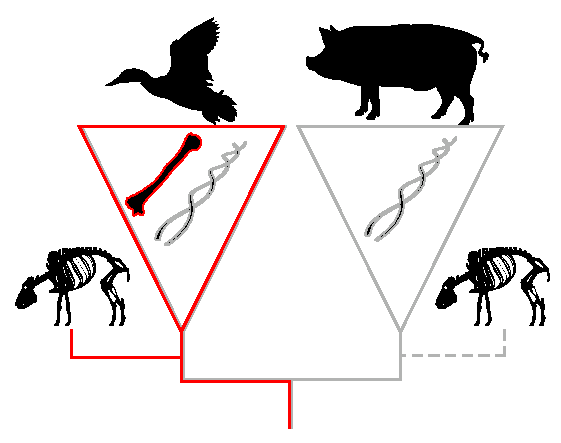
\includegraphics[width=1\textwidth]{MissingDataFigure.pdf}
%\caption{Example of topological errors due to missing morphological data in living taxa.
%The phylogeny contains two clades, Aves and Mammalia, with molecular data (grey) for both but only morphological data (red) for Aves.
%If a mammalian fossil species (with no molecular data) is added to the phylogeny, it will erroneously branch with the Aves instead of the Mammalia because no morphological data will overlap between the fossil mammals and the living ones.}
%\label{Figure_missing_data_problem}
%\end{figure}


\section{Supplementary results - 1}
The following section contains a supplementary analysis looking at the sampling effort for mammalian orders at three different taxonomic levels (family, genus and species).
We fitted linear regressions %TG: does one calculate regressions? I would go for drawing regressions but that's not semantically correct... % NC: It's a model so you fit it
between the log of the number of sampled families/genera/species for each order against the log of the total number of families/genera/species in each order % NC: Taken from where? The taxonomy? Where do you get this total from?
and fixed the intercept at zero (because when no families/genera/species exist they cannot be sampled).
The slope of the regression gives an indication of the sampling effort: if the slope is 1, the number of sampled families/genera/species and the total number of families/genera/species are equal, i.e. all families/genera/species have been sampled. 
Slopes of less than 1 indicate lower sampling effort.
The code for this analysis is available here: \url{github.com/TGuillerme/Missing_living_mammals/blob/master/Analysis/Sampling_effort.R}.

\begin{figure}[!htbp]
\centering
    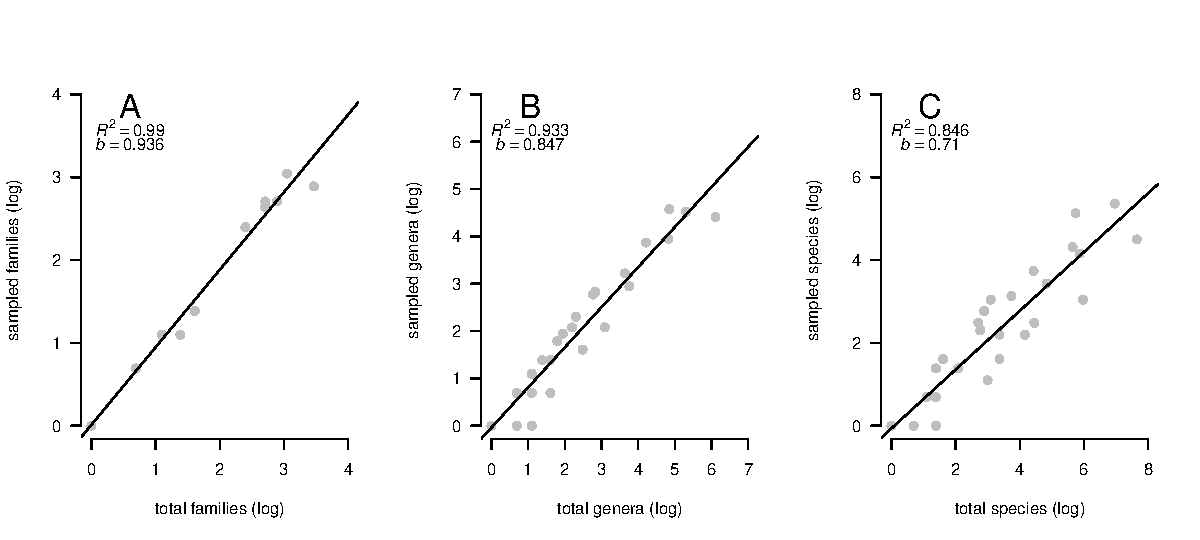
\includegraphics[width=1\textwidth]{Supp_figure_sampling_effort.pdf}
\caption{Sampling effort across mammalian orders at the three different taxonomic levels. The \textit{R$^2$} and the slope (\textit{b}, forced through the origin) are reported for each regression.} % NC: Should report adjusted r2 because sample size is small.
\label{Supp_Figure_sampling}
\end{figure}

% NC: Fix the y tick labels (use las = 1 to make them horizontal), what's up with panel c? the axes should be the same size as the others and why doesn't the x axis cover the range of the data? Also what are the three panels? explain in the legend and maybe label as a,b,c? Also axes labels should be log(sampled families) etc. 
%Supp mat is no excuse for sloppy figures.

This analysis suggests that sampling effort effectively reflects diversity for each taxonomic level, i.e. morphological characters were collected for each order according to its size (Figure \ref{Supp_Figure_sampling}).
However, it is worth noting that this relation is stronger at higher taxonomic levels (i.e. family-level, \textit{R$^2$}=0.99 \textit{b}=0.936) compared to the species-level (\textit{R$^2$}=0.852 \textit{b}=0.711).
These results might be simply due to the increasing number of groups at each taxonomic level (i.e. number of species $>$ genera $>$ families).
But it is also probable that mammalian morphological phylogeneticists have focused on resolving higher level relationships among mammalian orders (see Table 1 in the main text), resulting in better coverage at the family-level.

\newpage

\section{Supplementary results - 2}
The following section contains phylogenetic representations of availability of coded anatomical characters for each mammalian order (excluding results for Primates and Carnivora that are present in the main text).

\begin{figure}[!htbp]
\centering
    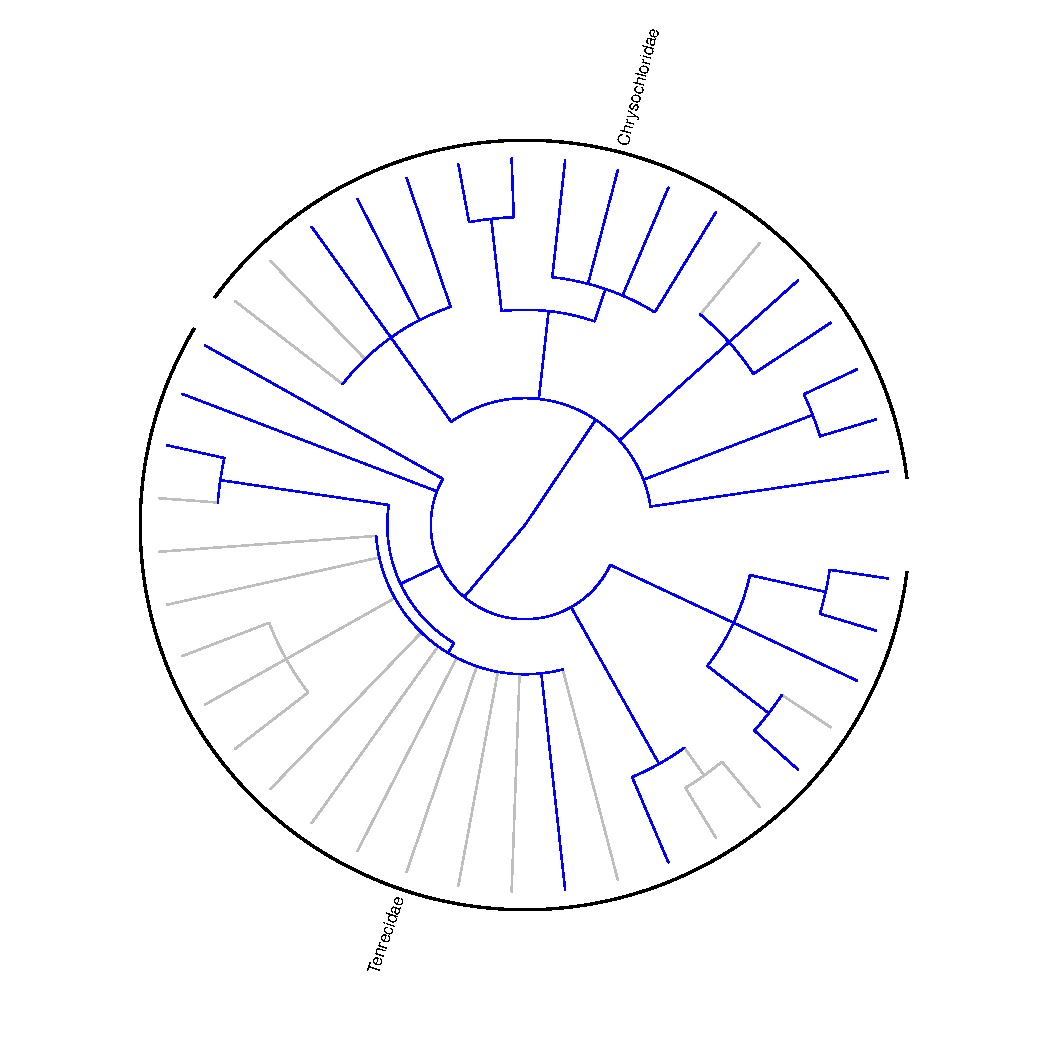
\includegraphics[width=1\textwidth]{Supp_figure_AFROSORICIDA.pdf}
\caption{Phylogenetic distribution of species with available coded anatomical characters across Afrosoricida. Blue branches indicate species with available coded anatomical characters.}
\label{Supp_Figure_Phylo-Afrosoricida}
\end{figure}

% NC: I have copied this wording from the main text. Fix all the ones below please :)

\begin{figure}[!htbp]
\centering
    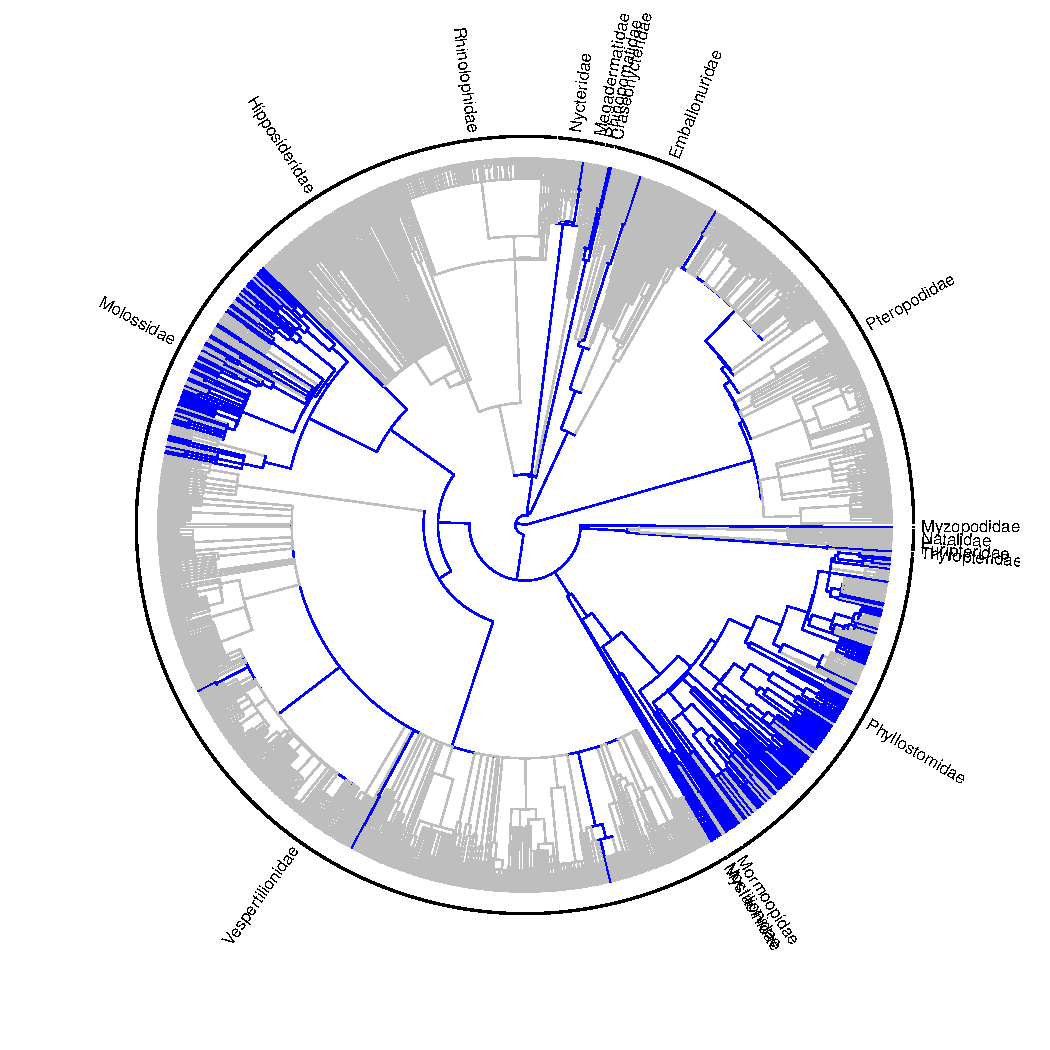
\includegraphics[width=1\textwidth]{Supp_figure_CHIROPTERA.pdf}
\caption{Distribution of available morphological data across Chiroptera. Edges are colored in grey when no morphological data is available or in blue when data is available.}
\label{Supp_Figure_Phylo-Chiroptera}
\end{figure}

\begin{figure}[!htbp]
\centering
    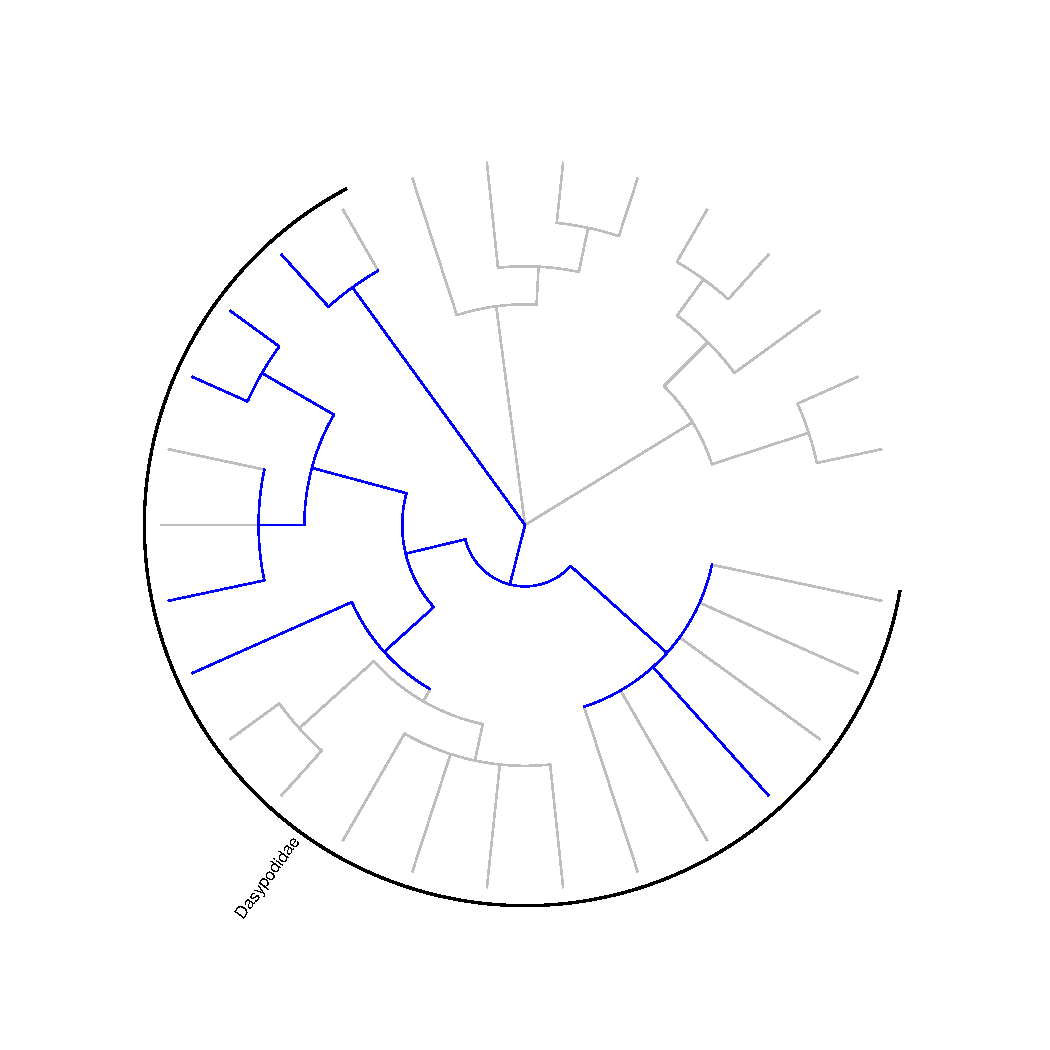
\includegraphics[width=1\textwidth]{Supp_figure_CINGULATA.pdf}
\caption{Distribution of available morphological data across Cingulata. Edges are colored in grey when no morphological data is available or in blue when data is available.}
\label{Supp_Figure_Phylo-Cingulata}
\end{figure}

\begin{figure}[!htbp]
\centering
    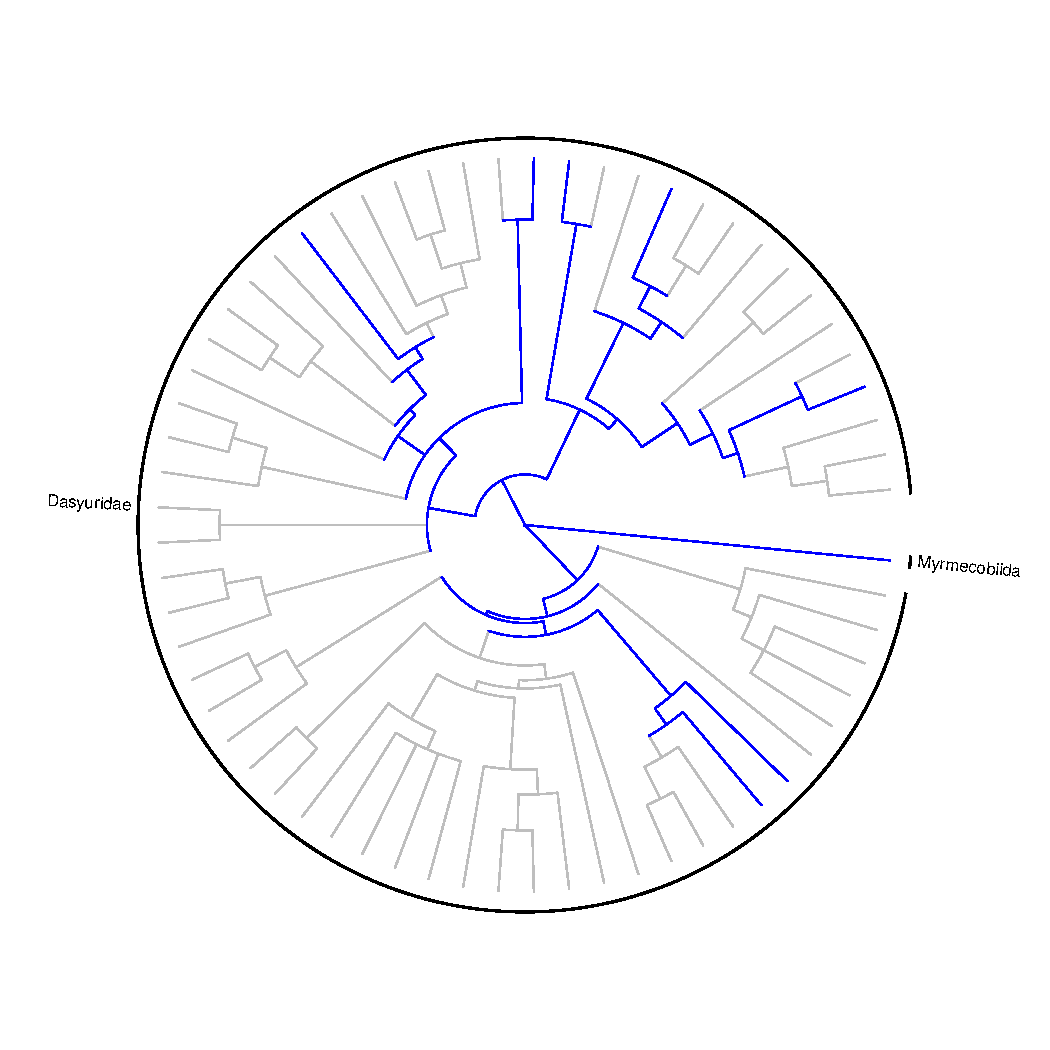
\includegraphics[width=1\textwidth]{Supp_figure_DASYUROMORPHIA.pdf}
\caption{Distribution of available morphological data across Dasyuromorphia. Edges are colored in grey when no morphological data is available or in blue when data is available.}
\label{Supp_Figure_Phylo-Dasyuromorphia}
\end{figure}

\begin{figure}[!htbp]
\centering
    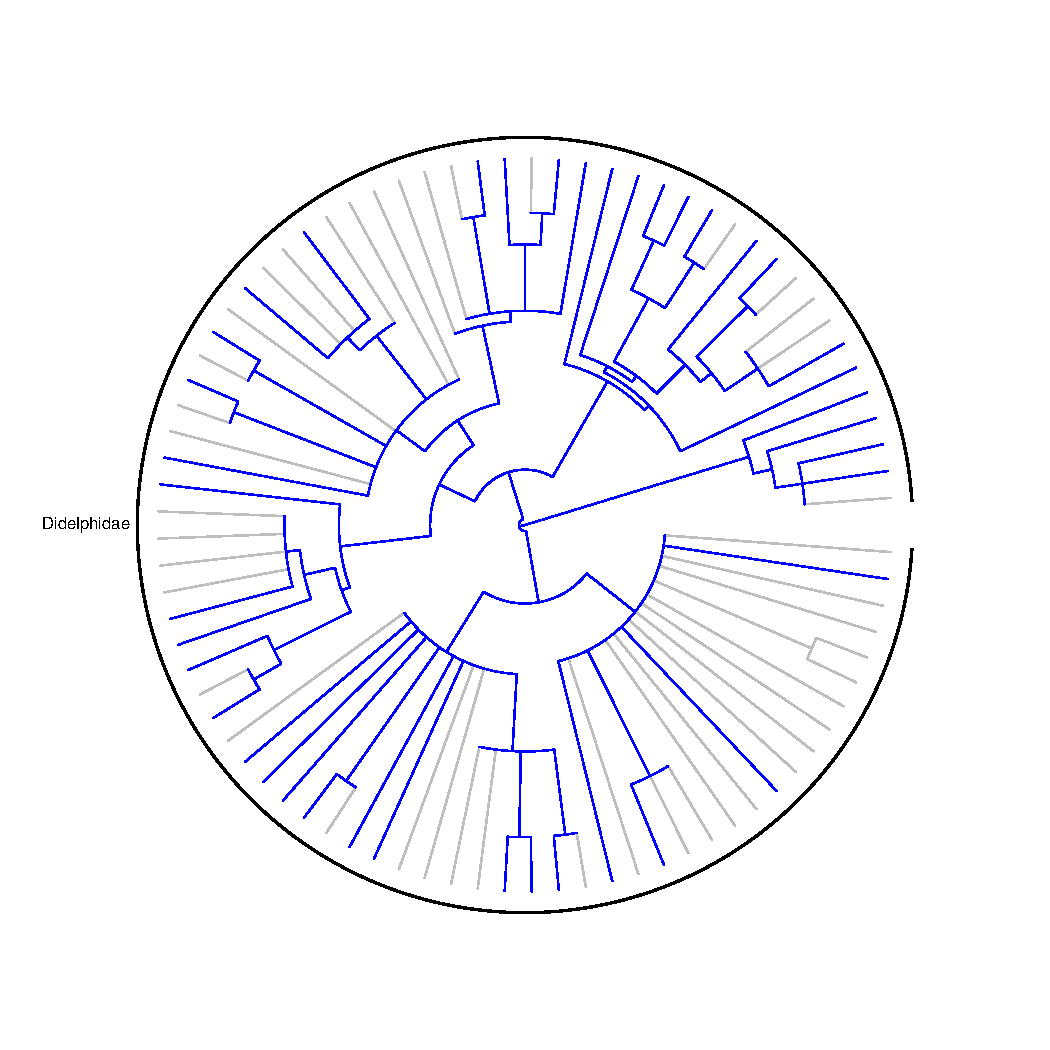
\includegraphics[width=1\textwidth]{Supp_figure_DIDELPHIMORPHIA.pdf}
\caption{Distribution of available morphological data across Didelphimorphia. Edges are colored in grey when no morphological data is available or in blue when data is available.}
\label{Supp_Figure_Phylo-Didelphimorphia}
\end{figure}

\begin{figure}[!htbp]
\centering
    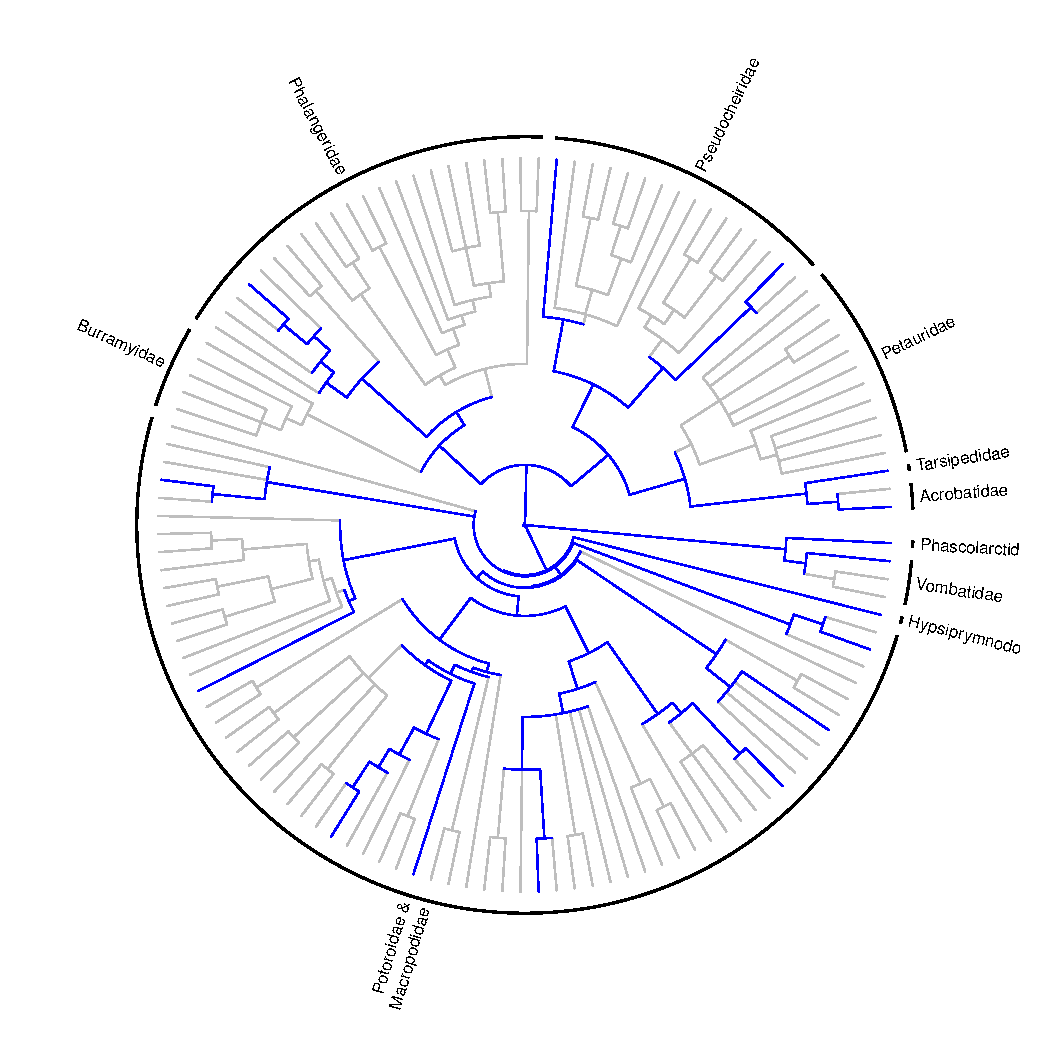
\includegraphics[width=1\textwidth]{Supp_figure_DIPROTODONTIA.pdf}
\caption{Distribution of available morphological data across Diprotodontia. Edges are colored in grey when no morphological data is available or in blue when data is available.}
\label{Supp_Figure_Phylo-Diprotodontia}
\end{figure}

\begin{figure}[!htbp]
\centering
    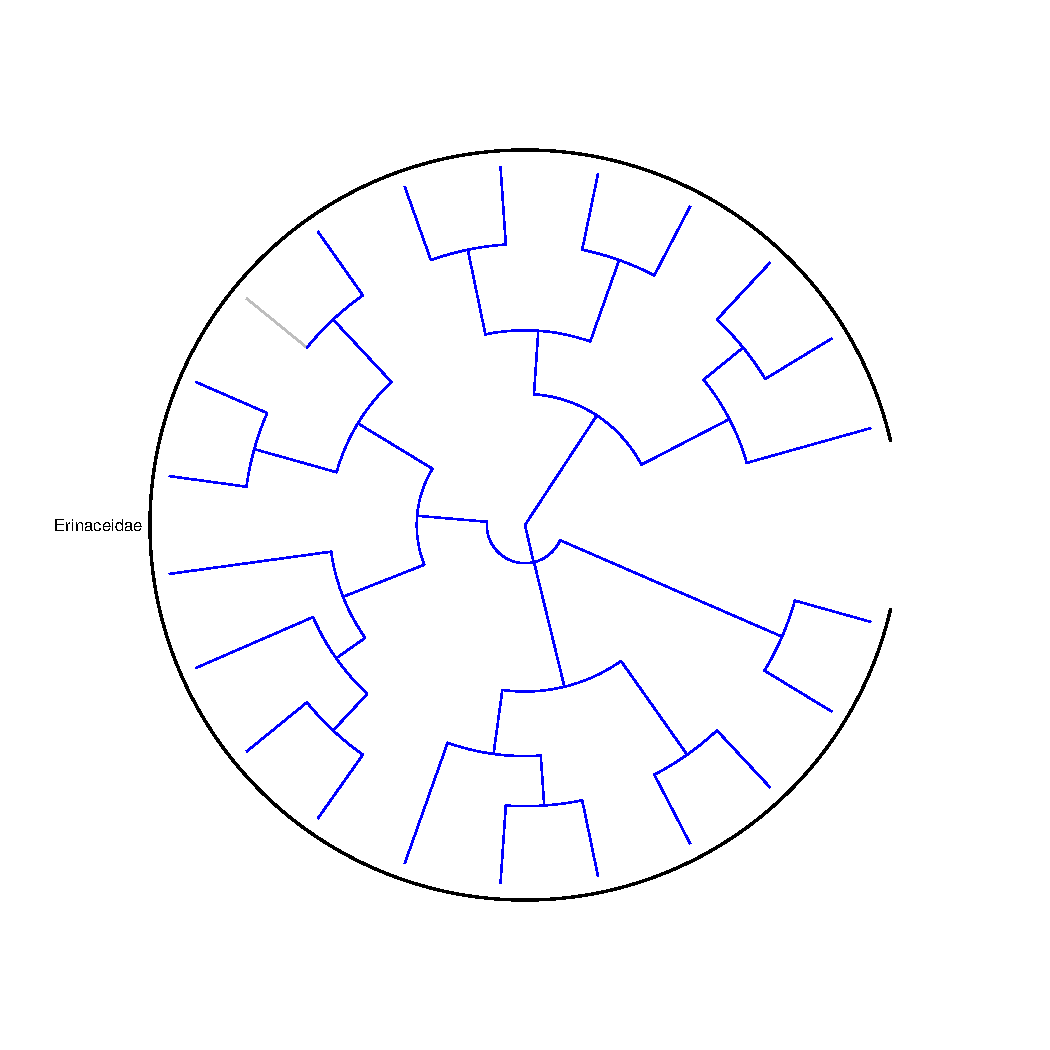
\includegraphics[width=1\textwidth]{Supp_figure_ERINACEOMORPHA.pdf}
\caption{Distribution of available morphological data across Erinaceomorpha. Edges are colored in grey when no morphological data is available or in blue when data is available.}
\label{Supp_Figure_Phylo-Erinaceomorpha}
\end{figure}

\begin{figure}[!htbp]
\centering
    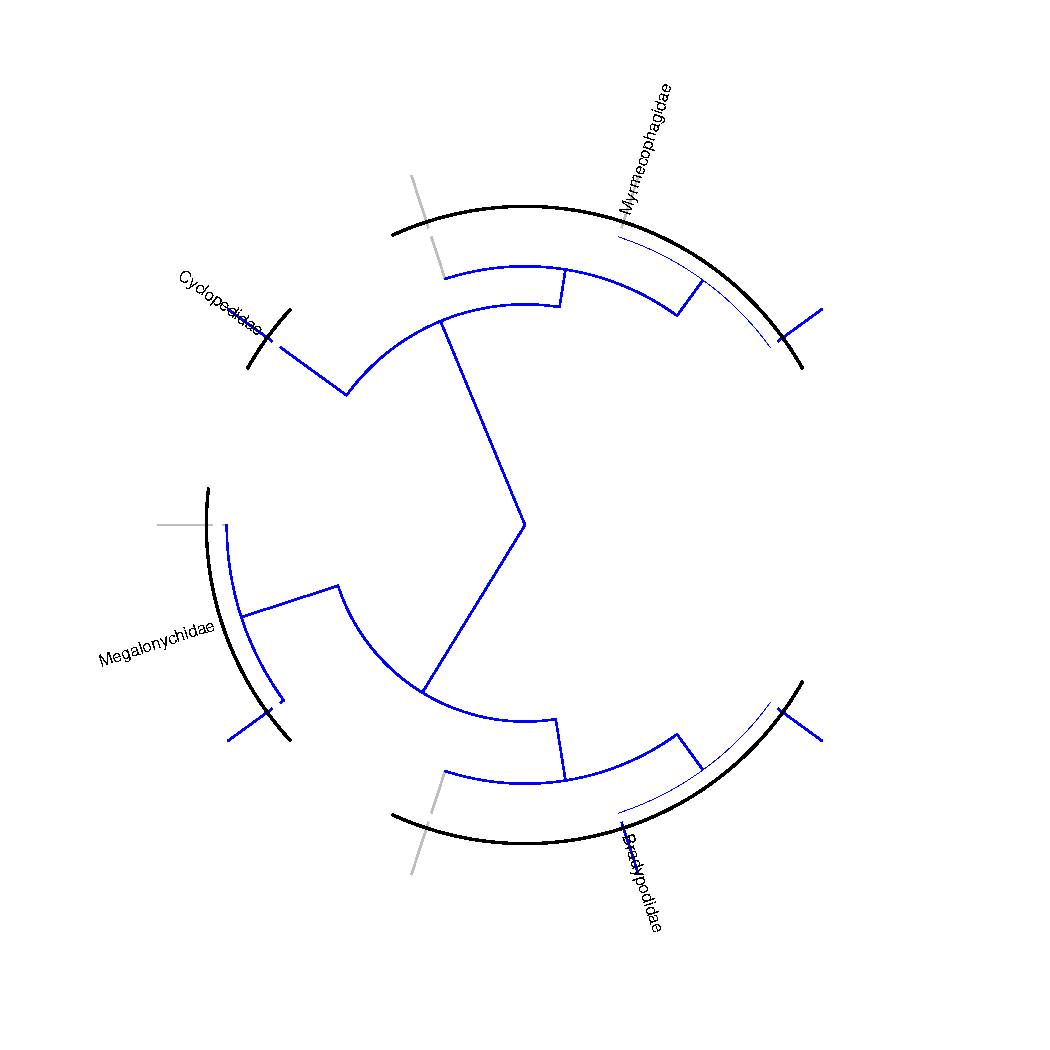
\includegraphics[width=1\textwidth]{Supp_figure_PILOSA.pdf}
\caption{Distribution of available morphological data across Pilosa. Edges are colored in grey when no morphological data is available or in blue when data is available.}
\label{Supp_Figure_Phylo-Pilosa}
\end{figure}

\begin{figure}[!htbp]
\centering
    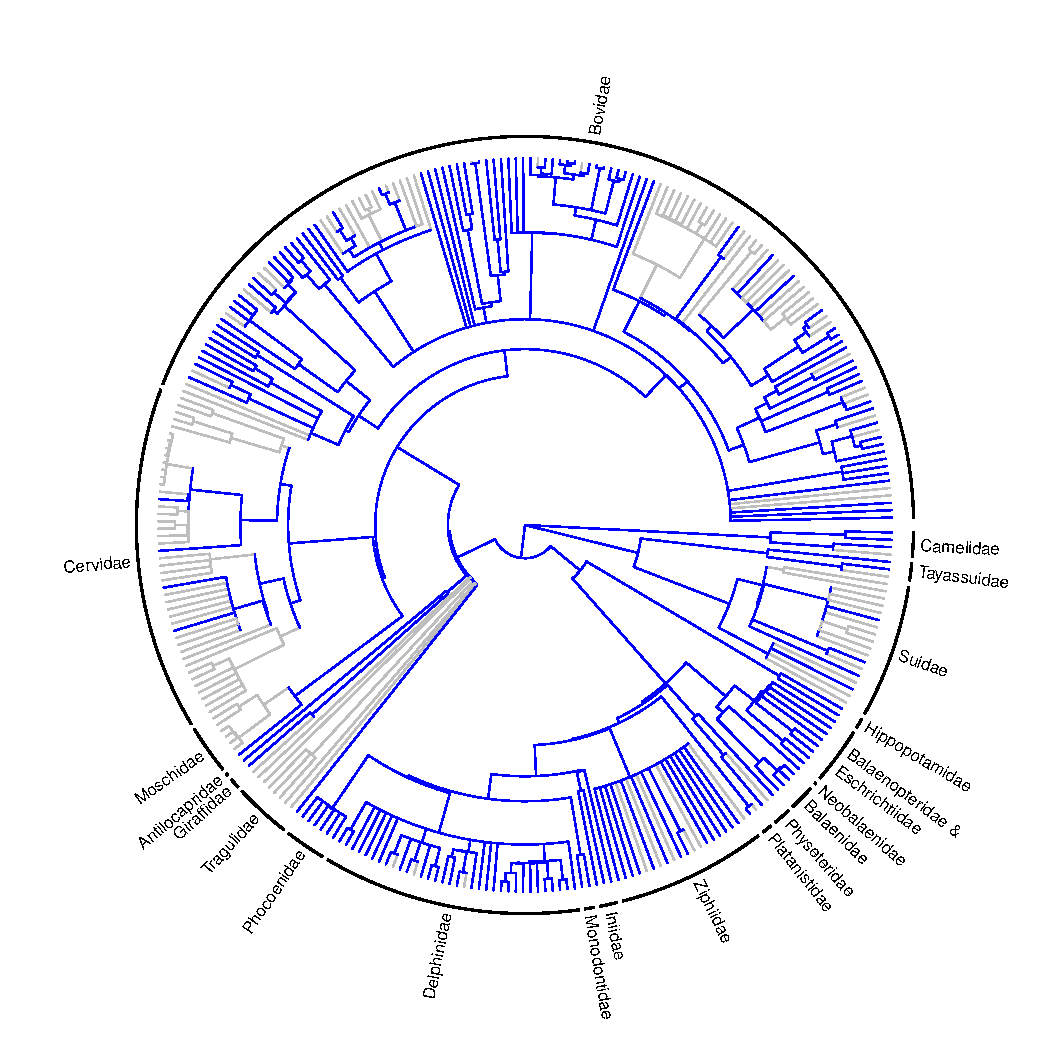
\includegraphics[width=1\textwidth]{Supp_figure_CETARTIODACTYLA.pdf}
\caption{Distribution of available morphological data across Cetartiodactyla. Edges are colored in grey when no morphological data is available or in blue when data is available.}
\label{Supp_Figure_Phylo-Primates}
\end{figure}

\begin{figure}[!htbp]
\centering
    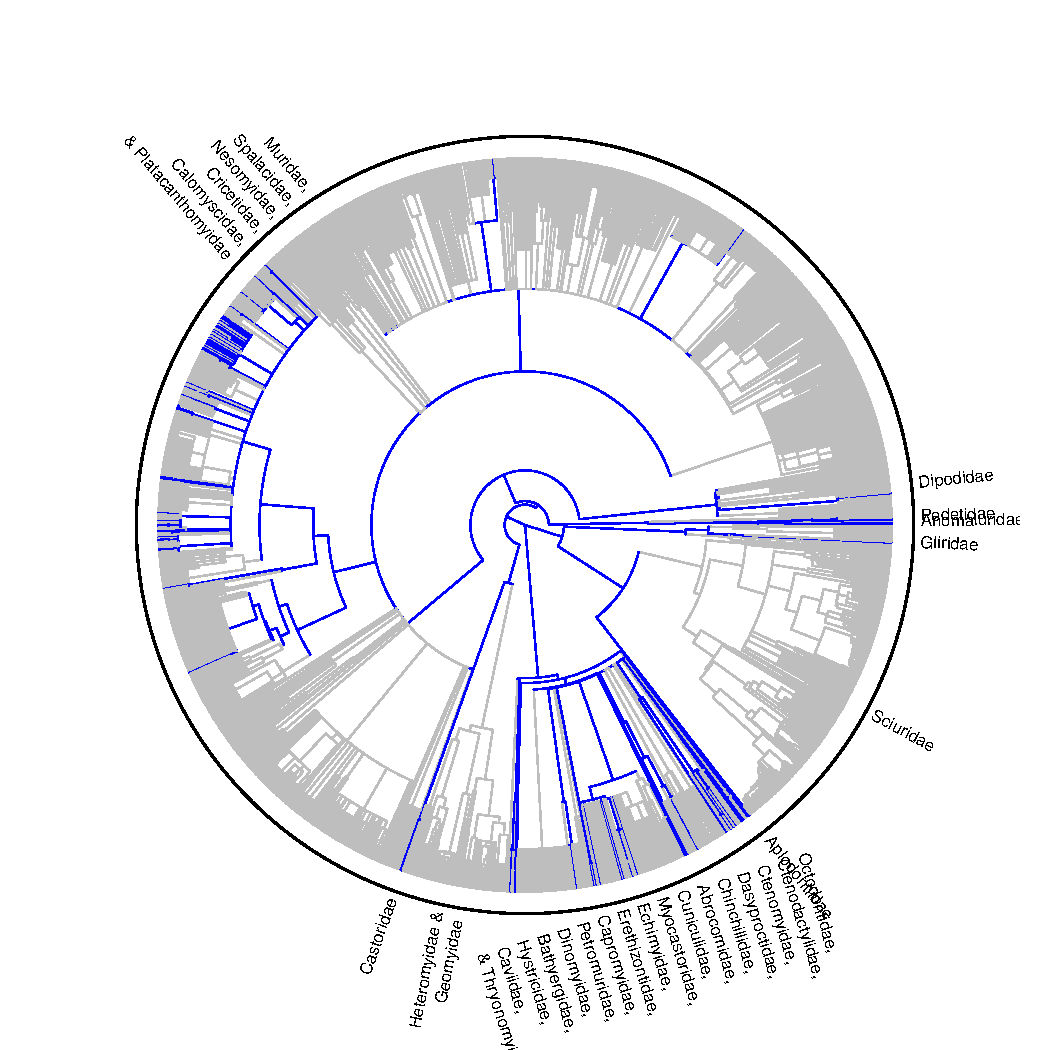
\includegraphics[width=1\textwidth]{Supp_figure_RODENTIA.pdf}
\caption{Distribution of available morphological data across Rodentia. Edges are colored in grey when no morphological data is available or in blue when data is available.}
\label{Supp_Figure_Phylo-Rodentia}
\end{figure}

\begin{figure}[!htbp]
\centering
    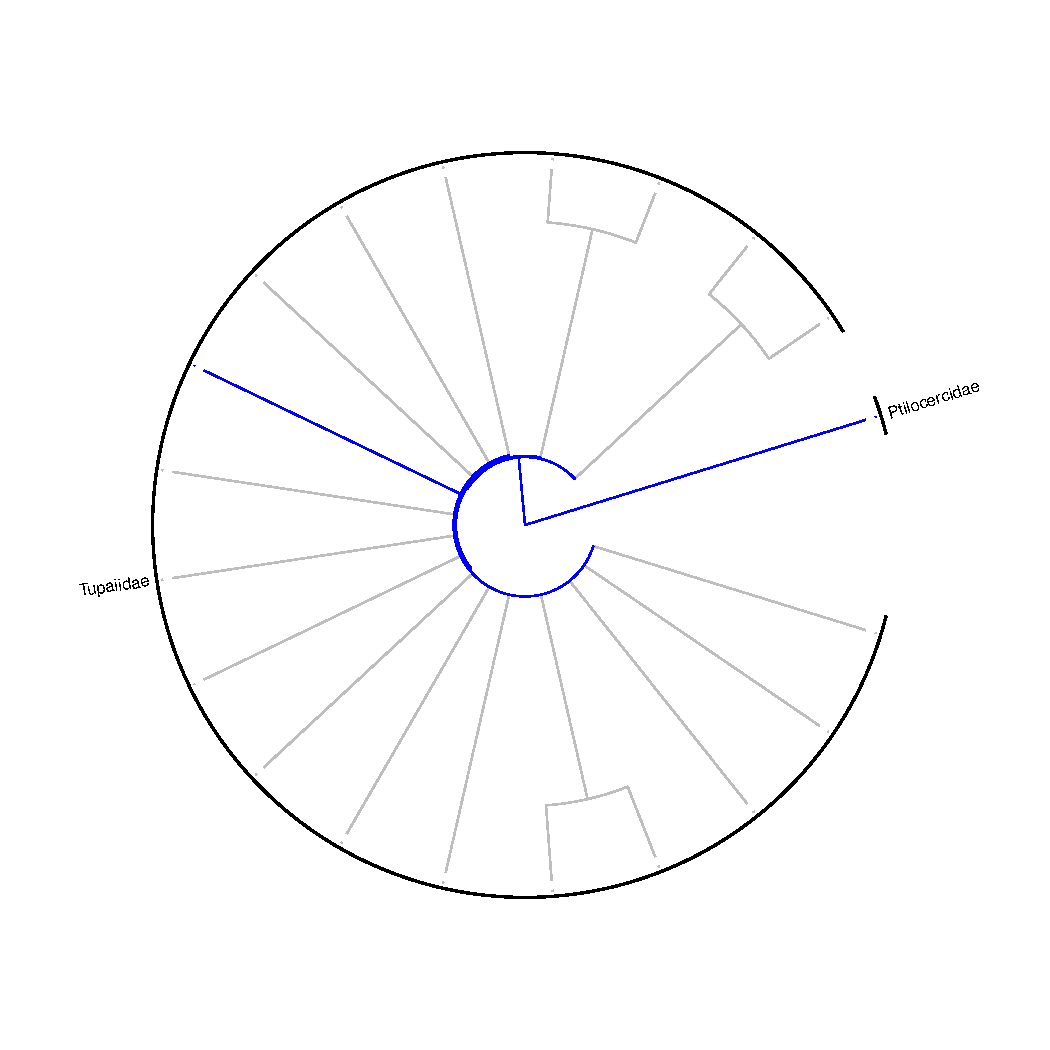
\includegraphics[width=1\textwidth]{Supp_figure_SCANDENTIA.pdf}
\caption{Distribution of available morphological data across Scandentia. Edges are colored in grey when no morphological data is available or in blue when data is available.}
\label{Supp_Figure_Phylo-Scandentia}
\end{figure}

\begin{figure}[!htbp]
\centering
    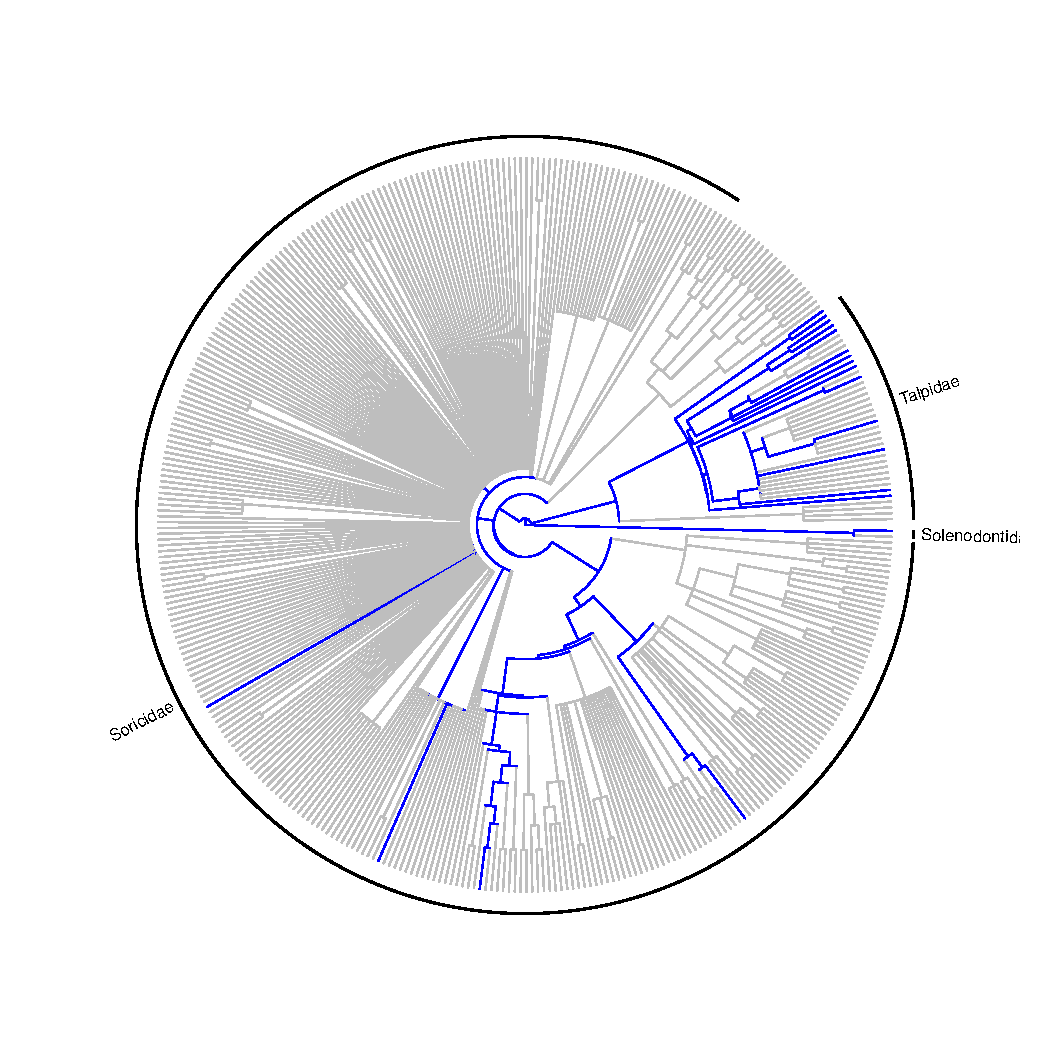
\includegraphics[width=1\textwidth]{Supp_figure_SORICOMORPHA.pdf}
\caption{Distribution of available morphological data across Soricomorpha. Edges are colored in grey when no morphological data is available or in blue when data is available.}
\label{Supp_Figure_Phylo-Soricomorpha}
\end{figure}


\end{document}